\documentclass[tikz,border=10pt]{standalone}
\usetikzlibrary{arrows.meta,positioning}

\begin{document}
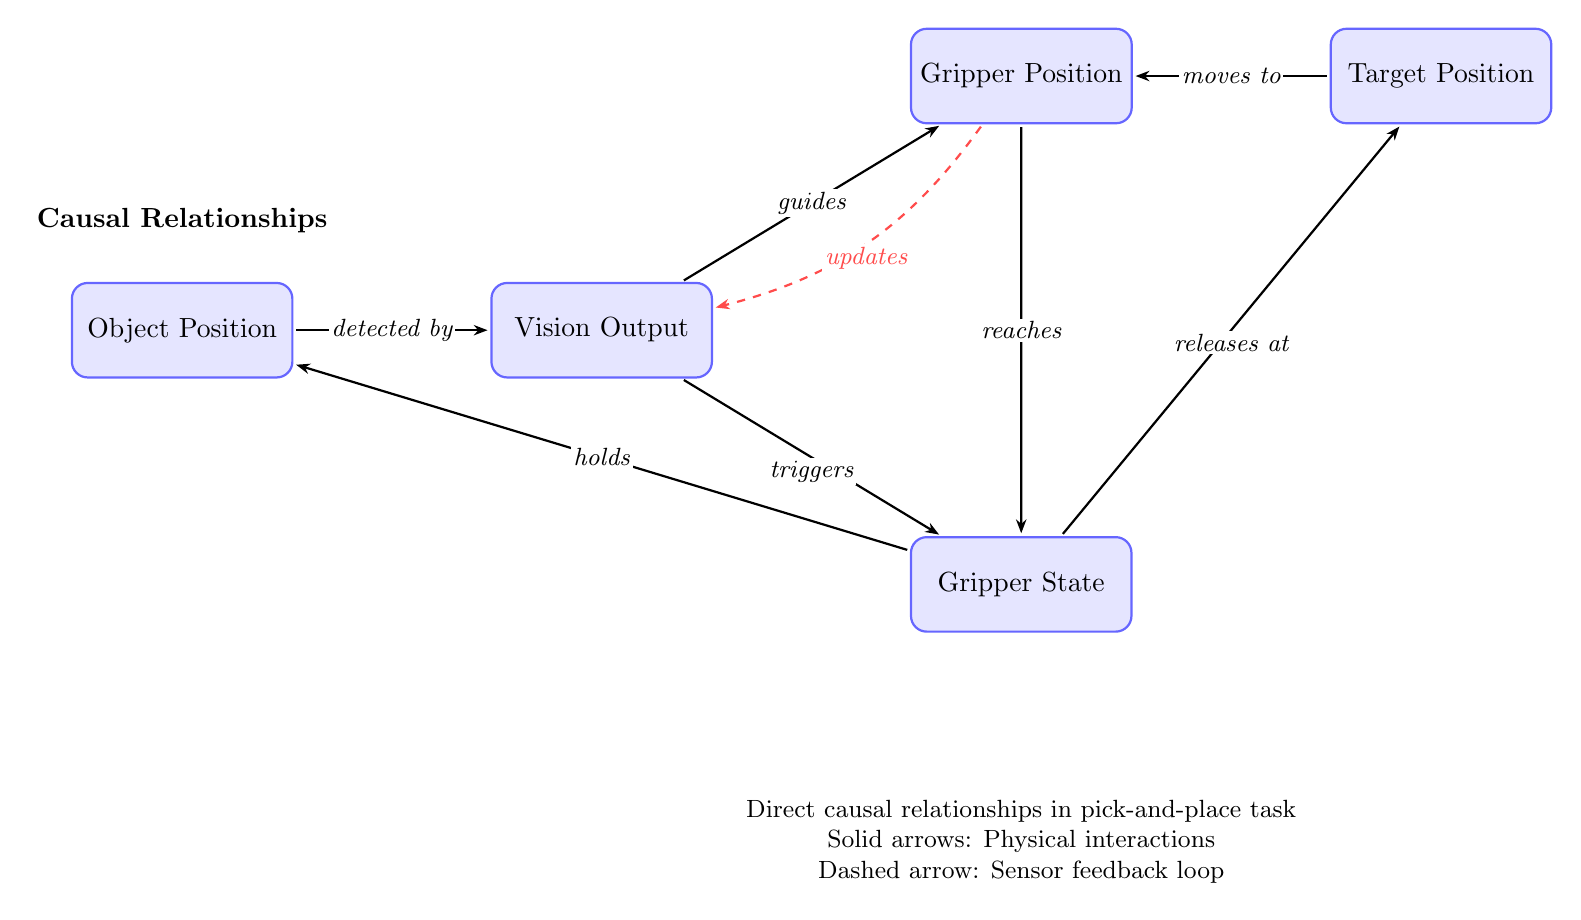
\begin{tikzpicture}[
    node distance=2cm and 2.5cm,
    var/.style={
        rectangle,
        draw=blue!60,
        fill=blue!10,
        thick,
        minimum width=2.8cm,
        minimum height=1.2cm,
        align=center,
        rounded corners=2mm
    },
    edge/.style={
        -{Stealth[length=5pt]},
        thick,
        shorten >=1pt,
        shorten <=1pt
    },
    label/.style={
        font=\itshape\small,
        midway,
        fill=white,
        inner sep=1pt
    }
]

% Nodes
\node[var] (obj_pos) {Object Position};
\node[var, right=of obj_pos] (vision) {Vision Output};
\node[var, above right=of vision] (grip_pos) {Gripper Position};
\node[var, below right=of vision] (grip_state) {Gripper State};
\node[var, right=of grip_pos] (target_pos) {Target Position};

% Edges with labels
\draw[edge] (obj_pos) -- node[label] {detected by} (vision);
\draw[edge] (vision) -- node[label] {guides} (grip_pos);
\draw[edge] (vision) -- node[label,below] {triggers} (grip_state);
\draw[edge] (grip_pos) -- node[label] {reaches} (grip_state);
\draw[edge] (target_pos) -- node[label] {moves to} (grip_pos);
\draw[edge] (grip_state) -- node[label,below] {releases at} (target_pos);
\draw[edge] (grip_state) -- node[label] {holds} (obj_pos);

% Feedback loop
\draw[edge, dashed, red!70] (grip_pos) to[bend left=20] node[label,below] {updates} (vision);

% Annotations
\node[above=0.5cm of obj_pos, font=\bfseries] {Causal Relationships};
\node[below=2cm of grip_state, align=center, font=\small] {
    Direct causal relationships in pick-and-place task\\
    Solid arrows: Physical interactions\\
    Dashed arrow: Sensor feedback loop
};

\end{tikzpicture}
\end{document}